\documentclass{article}
\usepackage{amssymb,amsmath}
\usepackage{ifxetex,ifluatex}
\ifxetex
  \usepackage{fontspec,xltxtra,xunicode}
  \defaultfontfeatures{Mapping=tex-text,Scale=MatchLowercase}
\else
  \ifluatex
    \usepackage{fontspec}
    \defaultfontfeatures{Mapping=tex-text,Scale=MatchLowercase}
  \else
    \usepackage[utf8]{inputenc}
  \fi
\fi
\usepackage{ctable}
\usepackage{float} % provides the H option for float placement
\usepackage{graphicx}
% We will generate all images so they have a width \maxwidth. This means
% that they will get their normal width if they fit onto the page, but
% are scaled down if they would overflow the margins.
\makeatletter
\def\maxwidth{\ifdim\Gin@nat@width>\linewidth\linewidth
\else\Gin@nat@width\fi}
\makeatother
\let\Oldincludegraphics\includegraphics
\renewcommand{\includegraphics}[1]{\Oldincludegraphics[width=\maxwidth]{#1}}
\ifxetex
  \usepackage[setpagesize=false, % page size defined by xetex
              unicode=false, % unicode breaks when used with xetex
              xetex]{hyperref}
\else
  \usepackage[unicode=true]{hyperref}
\fi
\hypersetup{breaklinks=true, pdfborder={0 0 0}}
\setlength{\parindent}{0pt}
\setlength{\parskip}{6pt plus 2pt minus 1pt}
\setlength{\emergencystretch}{3em}  % prevent overfull lines
\setcounter{secnumdepth}{0}

\title{Descriptives}
\author{Rapport package team @ https://github.com/aL3xa/rapport}
\date{2011--04--26 20:25 CET}

\begin{document}
\maketitle

\subsection{Description}

This template will return descriptive statistics of a numerical, or a
frequency table of a categorical variable.

\subsubsection{\emph{gender} (``Gender'')}

The dataset has 709 observations with 673 valid values (missing: 36) in
\emph{gender} (``Gender''). This variable seems to be a factor.

\paragraph{Base statistics}

\ctable[pos = H, center, botcap]{llllll}
{% notes
}
{% rows
\FL
 & \textbf{gender} & \textbf{N} & \textbf{pct} & \textbf{cumul.count} & \textbf{cumul.pct}
\ML
1 & male & 410.00 & 60.92 & 410.00 & 60.92
\\\noalign{\medskip}
2 & female & 263.00 & 39.08 & 673.00 & 100.00
\\\noalign{\medskip}
Total &  & 673.00 & 100.00 & 673.00 & 100.00
\LL
}

\paragraph{Barplot}

\begin{figure}[htbp]
\centering
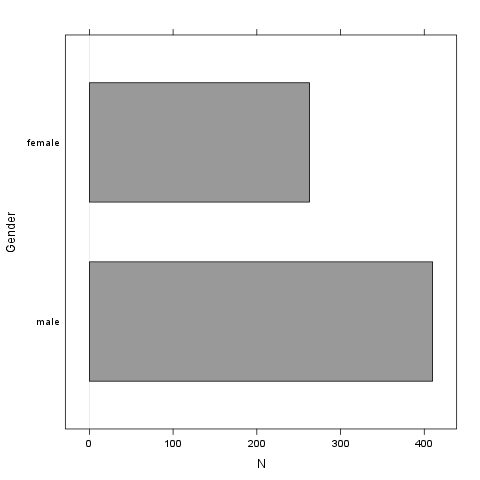
\includegraphics{3ed92ab3ffc6e875335e7e8c774c35a8.png}
\caption{}
\end{figure}

It seems that the highest value is 2 which is exactly 2 times higher
than the smallest value (1).

\subsection{Description}

This template will return descriptive statistics of a numerical, or a
frequency table of a categorical variable.

\subsubsection{\emph{age} (``Age'')}

The dataset has 709 observations with 677 valid values (missing: 32) in
\emph{age} (``Age''). This variable seems to be numeric.

\paragraph{Base statistics}

\ctable[pos = H, center, botcap]{llll}
{% notes
}
{% rows
\FL
\textbf{value} & \textbf{mean(age)} & \textbf{sd(age)} & \textbf{var(age)}
\ML
(all) & 24.57 & 6.85 & 46.91
\LL
}

\paragraph{Histogram}

\begin{figure}[htbp]
\centering
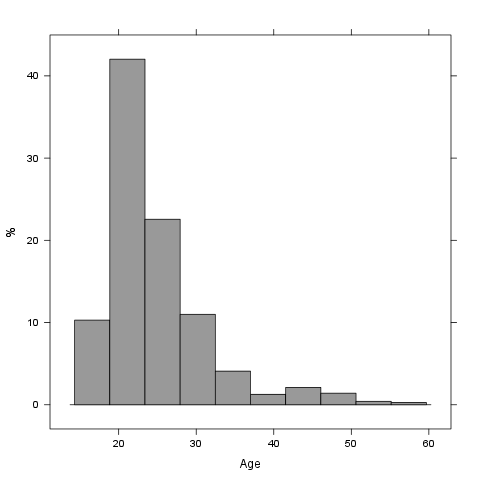
\includegraphics{ac5d789145bdef09b10219ef16429f53.png}
\caption{}
\end{figure}

It seems that the highest value is 58 which is exactly 3.625 times
higher than the smallest value (16).

The standard deviation is 6.8491 (variance: 46.911). The expected value
is around 24.573, somewhere between 24.057 and 25.089 (SE: 0.2632).

If we suppose that \emph{Age} is not near to a normal distribution
(test: , skewness: 1.9296, kurtosis: 7.4851), checking the median (23)
might be a better option instead of the mean. The interquartile range
(6) measures the statistics dispersion of the variable (similar to
standard deviation) based on median.

\end{document}
